\documentclass{beamer}

\usepackage[utf8]{inputenc}
\usepackage[T1]{fontenc}
\usepackage[ngerman]{babel}
\usepackage{graphicx} % Bilder
\usepackage{wrapfig} % Umflussbilder
\usepackage{multicol} % Multiple columns
\usepackage{minted} % Haskell source code
\usepackage{framed} % Frames around source code
\usepackage[framemethod=tikz]{mdframed} % Frames
\usepackage{verbatim} % \begin{comment}...\end{comment}
\usepackage{etoolbox} % manipulate minted
\AtBeginEnvironment{minted}{\fontsize{10}{10}\selectfont}
\AfterEndEnvironment{minted}{}

\mdfdefinestyle{fancy}{
  roundcorner=5pt,
  linewidth=4pt,
  linecolor=red!80,
  backgroundcolor=red!20
}
\newmdenv[style=fancy]{important}

% redifine \em for \emph to use bold instead of italics
\makeatletter
\DeclareRobustCommand{\em}{%
  \@nomath\em \if b\expandafter\@car\f@series\@nil
  \normalfont \else \bfseries \fi}
\makeatother

% Stuff for Beamer
\beamertemplatenavigationsymbolsempty
\usetheme{Warsaw}

\title{Fortgeschrittene Funktionale Programmierung in Haskell}

\begin{document}
  
%----------------------------------------------------------------------------------------  

  \begin{frame}
  \begin{center}
    \huge\textbf{Fortgeschrittene Funktionale Programmierung in Haskell}\\ \bigskip
    \LARGE Universität Bielefeld, Sommersemester 2015\\ \bigskip
    \large Jonas Betzendahl \& Stefan Dresselhaus
    \end{center}
  \end{frame}

%----------------------------------------------------------------------------------------  

\begin{frame}[allowframebreaks]{Outline}
\frametitle{Übersicht}
\tableofcontents
\end{frame}

%----------------------------------------------------------------------------------------

\begin{frame}

\textbf{Empfehlungen:}
\bigskip

\glqq Functionally Oblivious and Succinct\grqq\ - Edward Kmett\\
https://www.youtube.com/watch?v=WE2a90Bov0Q
\bigskip

\glqq Purely functiontional data structures\grqq\ - Chris Okasaki\\
www.cs.cmu.edu/~rwh/theses/okasaki.pdf
\bigskip

\begin{center}
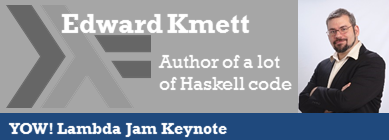
\includegraphics[scale=0.75]{../Woche8/kmett.png} 
\end{center}

\end{frame}

%----------------------------------------------------------------------------------------
\section{Vokabular und Wiederholung}
\begin{frame}
\Large
\begin{center}
Vokabular:\pause

Amortisation
\end{center}
\normalsize
\end{frame}
%----------------------------------------------------------------------------------------

\subsection{Vokabular: Amortisation}

\begin{frame}
\textbf{Remember big O?}
\bigskip

Ihr erinnert euch wahrscheinlich alle noch an Laufzeitanalysen mit der $\mathcal{O}$-Notation.
Hierbei wird die Größe des Eingabeproblems (z.B. Länge eines Arrays oder Anzahl Knoten in einem Graph, i.d.R. $n$) zur Anzahl der Rechenschritte zur Lösung des Problems in Verbindung gesetzt.
\pause
\bigskip

Dabei gibt es ein paar Dinge zu beachten:\pause

\begin{itemize}
\item Es wird (i.d.R.) nur die \emph{Laufzeit} betrachtet, und z.B. nicht, wie viel Speicher benötigt wird.\pause
\item Es wird nur die Laufzeit eines \emph{optimalen} Algorithmus zur Lösung des Problems betrachtet.\pause
\item Es wird nur die Verbindung zu einer \emph{Klasse} von Komplexität hergestellt. Konstante Faktoren werden ignoriert.\pause
\item Es wird nur das \emph{asymptotische} Wachstumsvehalten in der Zeit (also für \glqq unendlich\grqq\ große Eingaben) betrachtet.
\end{itemize}
\end{frame}

%----------------------------------------------------------------------------------------

\begin{frame}
\textbf{Das zweithäufigste Beispiel: Suchen}
\bigskip

Angenommen, wir haben eine Liste von $n$ Einträgen irgendeiner Art und wir suchen einen bestimmten davon.

Der Ansatz ist, dass wir von vorne jeden Eintrag einmal anschauen, überprüfen ob es unser Ziel ist, und im Zweifelsfall mit dem nächsten Element weiter machen.
\pause
\bigskip

Jetzt können verschiedene Dinge passieren:\pause

\begin{itemize}
\item \emph{best case:} Der Eintrag ist der erste in der Liste. Wir sind sofort fertig, ohne weitersuchen zu müssen.\pause
\item \emph{worst case:} Der Eintrag ist der letzte oder gar nicht in der Liste. Wir müssen die gesamte Liste durchgehen.\pause
\item \emph{average case:} Der Eintrag ist irgendwo sonst in der Liste. Im Schnitt müssen wir uns die Hälfte aller Elemente ansehen.
\end{itemize}

\end{frame}

%----------------------------------------------------------------------------------------

% Eventuell rausschneiden??

\begin{frame}
Ein paar typische Laufzeiten:

\begin{itemize}
\item $\mathcal{O}(1)$: Konstante Zeit\\
Feststellen, ob eine ganze Zahl gerade oder ungerade ist.\pause
\item $\mathcal{O}(\log{}n)$: Logarithmische Zeit\\
Binäre Suche\pause
\item $\mathcal{O}(n^2)$: Quadratische Zeit\\
Bubblesort, Insertion sort\pause
\item $\mathcal{O}(n^3)$: Kubische Zeit\\
Naive Matrizenmultiplikation\pause
\item $2^{\mathcal{O}(n)}$: Exponentielle Zeit\\
TSP mit der Magie dynamischer Programmierung\pause
\item $\mathcal{O}(n!)$: Faktorielle Zeit\\
TSP mit Brute-Force-Ansatz
\end{itemize}
\end{frame}

%----------------------------------------------------------------------------------------

\begin{frame}
Jetzt wollen wir unser Repertoire um ein neues Konzept erweitern:\smallskip\smallskip

\emph{Amortisierte} Laufzeitanalyse betrachtet nicht die asymptotische Laufzeit einer Operation unter bestimmten Annahmen (z.B. was ist der \glqq typische\grqq\ String?), sondern 
produziert eine Garantie, dass eine lange Sequenz von Operationen eine bestimmte Grenze nicht überschreitet.\pause\bigskip

Die amortisierten Kosten sind also \emph{nicht} (!) das Gleiche wie der average case. Letzterer ist eine Aussage über das Verhältnis von Eingabe und Laufzeit. Amortisierte Kosten beschreiben eine obere Grenze, die auf lange Sicht nicht überschritten wird, auch wenn einzelne Operationen darüber liegen können.
\end{frame}

%----------------------------------------------------------------------------------------

\begin{frame}
\textbf{Beispiel: Dynamisches Array}\bigskip

Man stelle sich ein Array vor, das wächst, wenn Elemente hinzugefügt werden. Lassen wir es mit der Größe vier starten.\pause\bigskip

Die ersten vier \texttt{push}-Operationen brauchen nur konstante Zeit ($\mathcal{O}(1)$). Die fünfte allerdings benötigt länger, weil jetzt erst ein neues Array (der Länge 8) angelegt werden muss und die Werte übertragen werden müssen ($\mathcal{O}(n)$), usw\dots
\pause\bigskip

Im Schnitt müssen wir also nur alle $n$ Operationen eine $\mathcal{O}(n)$-teure Operation durchführen, sonst konstant. Das bringt uns zu einer amortisierten Kostenfunktion $\mathcal{O}\left(\frac{n}{n}\right) = \mathcal{O}(1)$ für \texttt{push} auf dieser Sorte Array.
\end{frame}

%----------------------------------------------------------------------------------------

\begin{frame}
\begin{center}
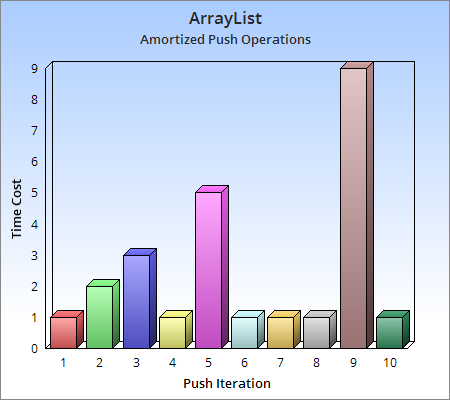
\includegraphics[scale=0.5]{AmortizedPush.png} 
\end{center}
\tiny
Bild: ScottDNelson, Wikipedia
\normalsize
\end{frame}

%----------------------------------------------------------------------------------------

\subsection{Wiederholung: Caches}

\begin{frame}
\Large
\begin{center}
Wiederholung(?):\\
Caches
\end{center}
\normalsize
\end{frame}

%----------------------------------------------------------------------------------------

\begin{frame}

\begin{wrapfigure}{r}{0.32\textwidth}
\vspace{-25pt}
 \begin{center}
   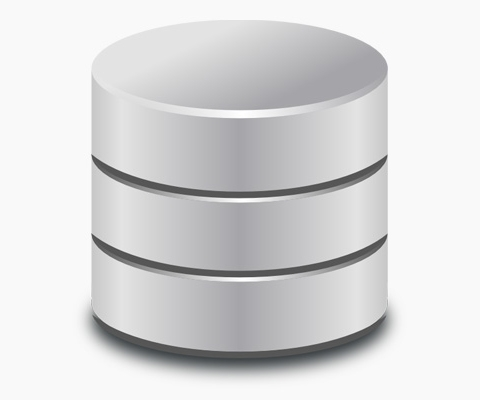
\includegraphics[width=0.34\textwidth]{ce_cache__full.jpg}
 \end{center}
 \vspace{-30pt}
 \end{wrapfigure}

Ein \emph{Cache} (vom franz. \emph{cacher}, verstecken) ist ein Zwischenspeicher, in den Ergebnisse (also Daten) gelegt werden können, um danach schnell (wiederholt) abgerufen zu werden statt aufwändig abgefragt oder neu berechnet zu werden.
\pause
\bigskip

Caches (realisiert sowohl Hardware als auch Software) gibt es in eurer CPU, auf eurer Festplatte, dazwischen, im Browser, auf Webservern, und auf gewisse Art sogar in eurem Gehirn.
\pause
\bigskip

Kann ein Ergebnis aus dem Cache verwendet werden, so nennt man das einen \emph{cache hit}, falls nicht, einen \emph{cache miss}.
\end{frame}

%----------------------------------------------------------------------------------------

\begin{frame}

\textbf{Tradeoff:} Size vs. Speed
\bigskip

\begin{center}

\includegraphics[scale=0.25]{browsercache.png} 
\end{center}

\end{frame}

%----------------------------------------------------------------------------------------

\begin{frame}

\textbf{Tradeoff:} Size vs. Speed
\bigskip

Jedes Mal wenn ein Datum angefragt wird, muss zunächst der Cache durchsucht werden, der dieses Datum enthalten könnte. Bei einem miss muss die nächste Ebene durchsucht werden, usw.
\pause
\bigskip

Caches in unseren Computern wachsen folglich exponentiell in sowohl ihrer Größe als auch in ihrer Langsamkeit (Latenz). Größere Caches sind also \emph{öfter}, dafür aber \emph{weniger} nützlich.

\end{frame}

%----------------------------------------------------------------------------------------

\begin{frame}

Zwischen eurem Code und der Festplatte liegen viele Caches\dots

\begin{center}
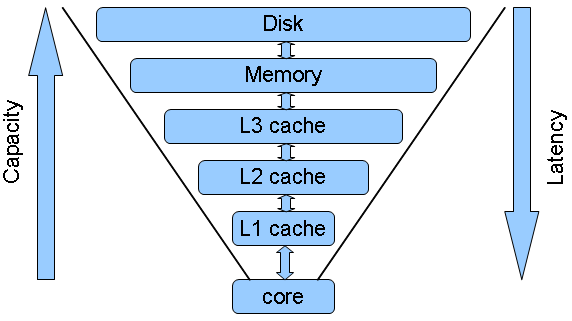
\includegraphics[scale=0.35]{cpu_cache_structure.png} 
\end{center}
\pause

\dots und ihr wisst nicht von allen, dass sie überhaupt existieren!

\end{frame}

%----------------------------------------------------------------------------------------
\subsection{Vokabular: Succinct data structures}
%----------------------------------------------------------------------------------------

\begin{frame}
\Large
\begin{center}
Vokabular:

Succinct data structures
\end{center}
\normalsize
\end{frame}

%----------------------------------------------------------------------------------------

\begin{frame}
foo bar baz
\end{frame}

%----------------------------------------------------------------------------------------
\section{cache-oblivious / succinct Data.Map}
%----------------------------------------------------------------------------------------

\begin{frame}
\Large
\begin{center}
cache-oblivious\\
succinct\\
\texttt{Data.Map}
\end{center}
\normalsize
\end{frame}
%----------------------------------------------------------------------------------------

\subsection{Was haben und was wollen wir?}

\begin{frame}[fragile]
\textbf{Was haben wir?}
\bigskip

Wir haben \texttt{Data.Map}, eine sehr gut gepflegte Bibliothek und der de-facto-Standard für
Performance-Benchmarks in Haskell.
\pause

Intern basiert alles auf \emph{trees of bounded balance}, welche wir hier allerdings nicht breit besprechen.\pause\bigskip

Exportiert eine reiche Auswahl an Funktionen:

\begin{minted}{haskell}
empty  :: Map k a -- construction
size   :: Map k a -> Int
member :: Ord k => k -> Map k a -> Bool
insert :: Ord k => k -> a -> Map k a -> Map k a 
lookup :: Ord k => k -> Map k a -> Maybe a 
map    :: (a -> b) -> Map k a -> Map k b 
...
union        :: Ord k => Map k a -> Map k a -> Map k a 
difference   :: Ord k => Map k a -> Map k b -> Map k a
intersection :: Ord k => Map k a -> Map k b -> Map k a 
...
\end{minted}
\end{frame}

%----------------------------------------------------------------------------------------

\begin{frame}
\textbf{Was hätten wir gerne?}
\pause
\bigskip
\begin{itemize}
\item hocheffiziente Variante einer \texttt{Map}\pause
\item insbesondere \emph{range queries} und \emph{inserts}\pause
\item Unterstützung für \emph{unboxed} data\\
      d.h. Datentypen, die einen direkten Wert darstellen und nicht einfach ein Pointer auf ein Objekt auf dem Heap sind.\pause
\item \dots während wir nicht die Nettigkeiten und Vorteile von \texttt{Haskell} aufgeben wollen.\pause
\end{itemize}

Was uns nicht so enorm wichtig ist, sind Anfragen nach genau einem Datenpunkt.\smallskip

Alles in allem sieht das etwas mehr nach einer Datenbank aus. Es ist aber insbesondere ein gutes Beispiel für das Konzept, was wir in Aktion sehen wollen.

\end{frame}
%----------------------------------------------------------------------------------------
\subsection{Memory Models}
%----------------------------------------------------------------------------------------

\begin{frame}
\textbf{Das IO-Model (damals):}

\begin{center}
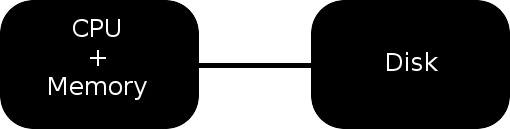
\includegraphics[scale=0.375]{model1.png} 
\end{center}
Sei hier $M$ die Größe des RAMs.\smallskip\smallskip
\pause

Eigenschaften dieses Modells:
\begin{itemize}
\item Wir können Blöcke der Größe $B$ lesen und schreiben\pause
\item Wir können max. $M/B$ Blöcke vorhalten, absolute Kontrolle\pause
\item Alle anderen Operationen sind \glqq umsonst\grqq
\end{itemize}
\end{frame}

%----------------------------------------------------------------------------------------

\begin{frame}
Dies erlaubt uns, \emph{optimale} Datenstrukturen für bestimmte $M$ zu finden, inklusive
hübscher Asymptoten:\pause\bigskip

$B$-Trees (nicht zu verwechseln mit binary trees):
\begin{center}
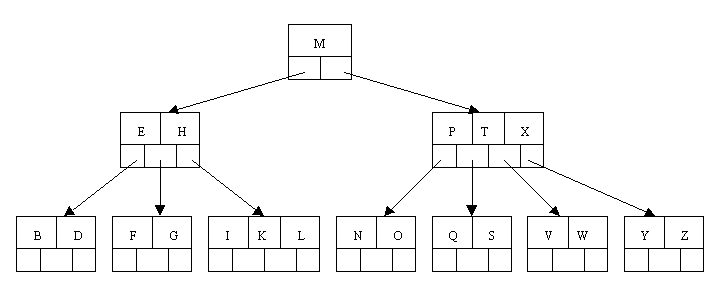
\includegraphics[scale=0.35]{btree1.png}
\end{center}
\pause

\begin{itemize}
\item Belegt $\mathcal{O}(\frac{N}{B})$ Blöcke Speicher
\item Update möglich in $\mathcal{O}(\log{}\frac{N}{B})$
\item Suche möglich in $\mathcal{O}(\log{\left(\frac{N}{B}\right)} + \frac{a}{B})$ wobei $a$ Resultatgröße
\end{itemize}
\end{frame}

%----------------------------------------------------------------------------------------

\begin{frame}

Dieses Modell gibt uns zwar viel schönes, weil wir direkte Kontrolle über den einen Cache haben, es gibt aber zwei Probleme damit:\pause

\begin{itemize}
\item Wenn wir die Architektur wechseln müssen wir von vorne anfangen, unsere Konstanten abzustimmen.\pause
\item Das ist nicht, wie heutige Rechner tatsächlich aussehen.\pause
\end{itemize}
\bigskip

\begin{center}
\emph{All models are wrong but some are useful. This one isn't.}
\end{center}
\end{frame}

%----------------------------------------------------------------------------------------

\begin{frame}
\textbf{Realistischer: Das IO-Model (\glqq gestern\grqq):}

\begin{center}
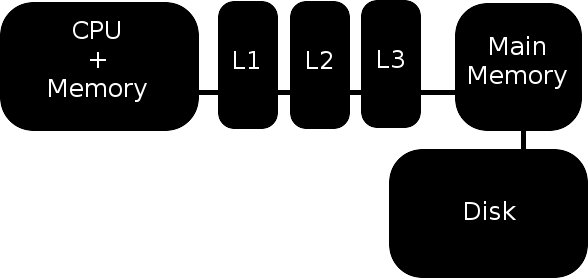
\includegraphics[scale=0.325]{model2.png} 
\end{center}
Sei hier $M$ wieder die Größe des RAMs. Oder besser $M_1$, $M_2$, \dots\smallskip\smallskip
\pause

Probleme:
\begin{itemize}
\item Jede Menge Konstanten abzustimmen, sehr viel Arbeit\pause
\item Optimierung für einen Cache suboptimiert für andere!\pause
\item Fordert Unmengen an Gehirnpower und Fachwissen 
\end{itemize}
\end{frame}

%----------------------------------------------------------------------------------------

\begin{frame}
\textbf{Deswegen: Das Cache-Oblivious-Model (heute):}

\begin{center}
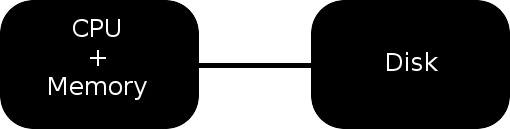
\includegraphics[scale=0.325]{model1.png} 
\end{center}
\pause

\begin{multicols}{2}
Erstmal wie gehabt:\smallskip\smallskip

\begin{itemize}
\item Kann Blöcke der Größe $B$ lesen und schreiben
\item Kann $\frac{M}{B}$ Blöcke vorhalten
\item Alle anderen Operationen sind \glqq umsonst\grqq
\end{itemize}

\columnbreak
\pause

ABER:

Wir kennen weder $M$, noch $B$! \smallskip\smallskip
\pause

\begin{itemize}
\item Asymp. optimale Alg. für unbekannte Größen sind asymp. optimal für \emph{alle} Caches!\pause
\item \dots gegeben ein Orakel mit perfekter \emph{eviction policy}.
\end{itemize}

\end{multicols}
\end{frame}

%----------------------------------------------------------------------------------------
\subsection{Zahlensysteme}
%----------------------------------------------------------------------------------------

\begin{frame}
Bisher haben wir uns nur mit dem \emph{Auslesen} unserer super-simplen Datenstruktur von
vorhin beschäftigt\dots Aber was ist mit dem \emph{Einfügen} von Daten?\pause\bigskip

Netterweise haben uns Bentley und Saxe in 1980 bereits einen Weg gegeben (genannt das \emph{Bentley-Saxe dynamisation scheme}):\pause
\begin{itemize}
\item Man nehme: Verlinkte Liste einer beliebigen flachen Datenstruktur\pause
\item Jedes Element hat Größe von aufsteigenden Zweierpotenzen\pause
\item Die Liste ist aufsteigend nach Größe sortiert
\end{itemize}
\end{frame}

%----------------------------------------------------------------------------------------

\begin{frame}
\textbf{Bentley-Saxe:}
\begin{center}
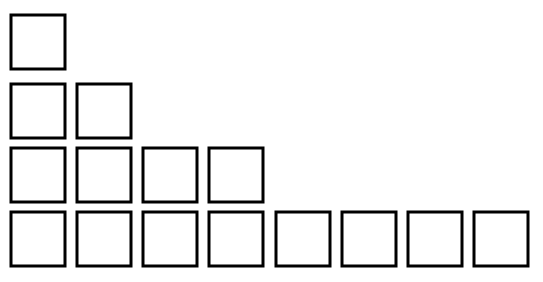
\includegraphics[scale=0.5]{bentley_saxe_00.png} 
\end{center}

Wie oben besprochen\dots
\end{frame}

%----------------------------------------------------------------------------------------

\begin{frame}
\textbf{Bentley-Saxe:}
\begin{center}
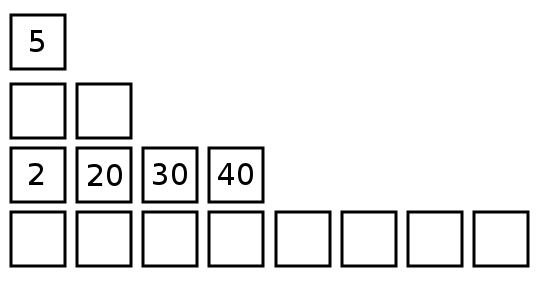
\includegraphics[scale=0.5]{bentley_saxe_01.png} 
\end{center}

Jetzt gefüllt mit ein paar Daten.
\end{frame}

%----------------------------------------------------------------------------------------

\begin{frame}
\textbf{Bentley-Saxe:}
\begin{center}
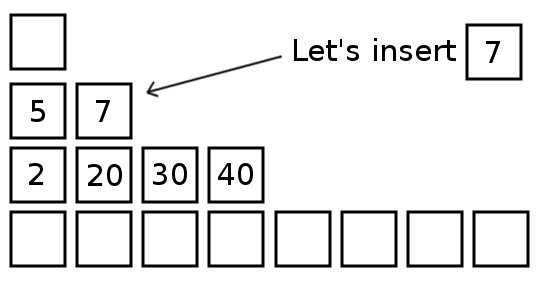
\includegraphics[scale=0.5]{bentley_saxe_02.png} 
\end{center}

Wenn wir 7 einfügen, rutscht 5 in die größere Liste und merged.
\end{frame}

%----------------------------------------------------------------------------------------

\begin{frame}
\textbf{Bentley-Saxe:}
\begin{center}
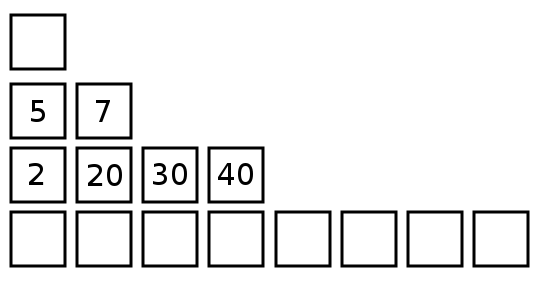
\includegraphics[scale=0.5]{bentley_saxe_03.png} 
\end{center}

Wir haben außerdem \glqq gezählt\grqq . Von $101$ zu $110$ 
\end{frame}

%----------------------------------------------------------------------------------------

\begin{frame}
\textbf{Bentley-Saxe:}
\begin{center}
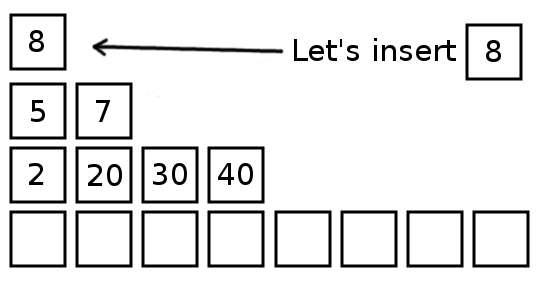
\includegraphics[scale=0.5]{bentley_saxe_04.png} 
\end{center}

Dieser Insert benötigt keinen gesonderten Mergevorgang.
\end{frame}

%----------------------------------------------------------------------------------------

\begin{frame}
\textbf{Bentley-Saxe:}
\begin{center}
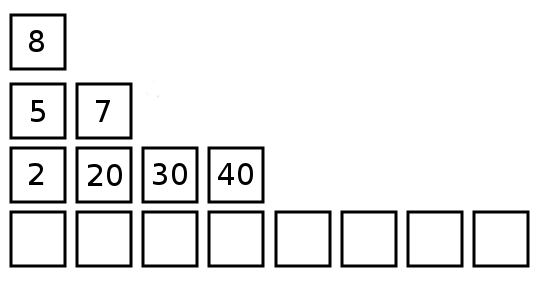
\includegraphics[scale=0.5]{bentley_saxe_05.png} 
\end{center}

Was gibt uns das für Asymptoten?
\end{frame}

%----------------------------------------------------------------------------------------

\begin{frame}
\textbf{Bentley-Saxe:}
\begin{center}
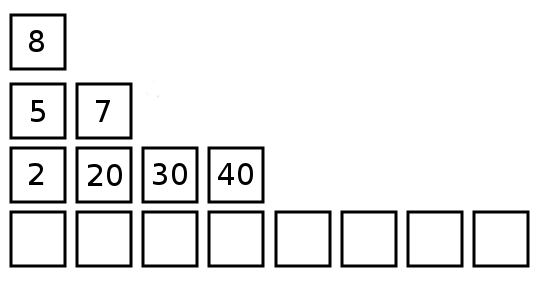
\includegraphics[scale=0.25]{bentley_saxe_05.png} 
\end{center}

Was gibt uns das für Asymptoten?\bigskip

\begin{itemize}
\item worst-case insert liegt in $\mathcal{O}(\frac{N}{B})$\pause
\item amortisiertes insert liegt in $\mathcal{O}(\frac{\log{}N}{B})$\pause
\end{itemize}

Das gleiche Ergebnis wie im \glqq optimalen\grqq\ $B$-Tree, das allerdings \emph{ohne $B$ zu kennen!}
\end{frame}

%----------------------------------------------------------------------------------------

\begin{frame}
Sloppy and dysfunctional
\end{frame}

%----------------------------------------------------------------------------------------

\begin{frame}
\textbf{Zeroless Binary:}

\begin{multicols}{2}

\begin{tabular}{c|c}
Dezimal & ZL Binary \\ 
\hline
&\\
0&000\\
1&001\\
2&002\\
3&011\\
4&012\\
5&021\\
6&022\\
7&111\\
8&112\\
9&121\\
10&122\\
\end{tabular}
\columnbreak
\pause

\begin{itemize}
\item Alle Ziffern sind 1 oder 2 (nur führende 0en erlaubt)\pause
\item Stellenwerte aus dem Binärsystem ($2^0, 2^1, 2^2$\dots) werden beibehalten\pause
\item Es existiert eine eindeutige Darstellung, Zahlen sind also unambiguitiv darstellbar\pause
\item \dots und trotzdem noch immmer nicht das, was wir suchen.
\end{itemize}

\end{multicols}
\end{frame}

%----------------------------------------------------------------------------------------

\begin{frame}
\textbf{\emph{Modified} Zeroless Binary:}

\begin{multicols}{2}

\begin{tabular}{c|c}
Dezimal & Modified ZLB \\ 
\hline
&\\
0&000\\
1&001\\
2&002\\
3&003\\
4&012\\
5&013\\
6&022\\
7&023\\
8&032\\
9&033\\
10&122\\
\end{tabular}
\columnbreak
\pause

\begin{itemize}
\item Alle Ziffern sind 1, 2 oder 3\pause
\item Nur an vorderster Stelle darf eine 1 stehen\pause
\item Stellenwerte aus dem Binärsystem ($2^0, 2^1, 2^2$\dots) werden beibehalten\pause
\item Es existiert eine eindeutige Darstellung\pause
\item Hat genau die richtige Menge an Verzögerung!
\end{itemize}

\end{multicols}
\end{frame}

%----------------------------------------------------------------------------------------

\begin{frame}
\textbf{Vergleich der Zahlensysteme:}
\smallskip\smallskip

\begin{center}
\begin{tabular}{c|c|c|c}
Dezimal & Binary & ZL Binary & Modified ZLB\\ 
\hline
   &      &     &    \\
0  & 0000 & 000 & 000\\
1  & 0001 & 001 & 001\\
2  & 0010 & 002 & 002\\
3  & 0011 & 011 & 003\\
4  & 0100 & 012 & 012\\
5  & 0101 & 021 & 013\\
6  & 0110 & 022 & 022\\
7  & 0111 & 111 & 023\\
8  & 1000 & 112 & 032\\
9  & 1001 & 121 & 033\\
10 & 1010 & 122 & 122\\
\end{tabular}
\end{center}

\end{frame}

%----------------------------------------------------------------------------------------

\begin{frame}[fragile]

\textbf{Why the *bleep* do we care?!}
\pause
\bigskip

Because now we have this:

\begin{minted}[fontsize=\scriptsize]{haskell}
data Map k a
  = M0 
  | M1 !(Chunk k a) 
  | M2 !(Chunk k a) !(Chunk k a) (Chunk k a) !(Map k a)
  | M3 !(Chunk k a) !(Chunk k a) !(Chunk k a) (Chunk k a) !(Map k a)
  
data Chunk k a = Chunk !(Array k) !(Array a)

-| O(log(N)/B) persistently amortised. insert an element.
insert :: (Ord k, Arrayed k, Arrayed v) => k -> v -> Map k v -> Map k v
insert k0 v0 = g0 $ Chunk (singleton k0) (singleton v0) where
  go as M0                 = M1 as
  go as (M1 bs)            = M2 as bs (merge as bs) M0
  go as (M2 bs cs bcs xs)  = M3 as bs cs bcs xs
  go as (M3 bs _ _ cds xs) = cds `seq` M2 as bs (merge as bs) (go cds xs)
{-# INLINE insert #-}
\end{minted}
%$

\end{frame}

\begin{frame}
\textbf{Why the *bleep* do we care?! (2)}
\pause
\bigskip

\begin{itemize}
\item \texttt{insert} ist jetzt 7-10x schneller als Äquivalent aus \texttt{Data.Map} und wird beim Skalieren nur schneller\pause
\item Wir können eine unboxed map bauen, wenn wir unboxed Datentypen reinstecken.\pause
\item Asymp. $B$-Tree performance ohne $B$ kennen zu müssen.\pause
\item Keine Konstanten, die wir feinabstimmen müssten.
\end{itemize}
\end{frame}

%----------------------------------------------------------------------------------------

\end{document}